\documentclass[runningheads]{llncs}

\usepackage[T1]{fontenc}
\usepackage[utf8]{inputenc}
\usepackage{graphicx}
\usepackage{amsmath,amssymb}
\usepackage{booktabs}
\usepackage{url}
\usepackage{algorithm}
\usepackage{algpseudocode}
\usepackage{multirow}
\usepackage{colortbl}

\begin{document}

\title{Dynamic Graph Learning with Temporal Attention for Portfolio Optimization in the Vietnam Stock Market}

\author{Trong Hieu Tran\inst{1} \and
       Dinh Hai Luong\inst{2} \and
       Thi Hong Khanh Nguyen\inst{3}}

\institute{
    Faculty of Information Technology, VNU University of Engineering and Technology, Hanoi, Vietnam\\
    \email{hieutt@vnu.edu.vn}
    \and
    Faculty of Mathematics, Mechanics and Informatics, VNU University of Science, Hanoi, Vietnam\\
    \email{24007802@hus.edu.vn}
    \and
    Faculty of Information Technology, Electric Power University, Hanoi, Vietnam\\
    \email{khanhnth@epu.edu.vn}
}

\maketitle

\begin{abstract}
Portfolio optimization is a challenging problem due to the dynamic dependencies among financial assets and the uncertainty of market conditions. This paper proposes a hybrid framework that integrates Graph Neural Networks (GNNs) and Reinforcement Learning (RL) for portfolio optimization in the Vietnamese stock market. The proposed method models inter-stock relationships using a graph attention network over a correlation graph that is re-estimated at every rebalancing date, and incorporates a Transformer-based temporal attention encoder to capture historical market dynamics. The resulting graph representations are combined with a Proximal Policy Optimization (PPO) agent, trained end-to-end against a transaction-cost-aware, Sharpe-based reward, to generate portfolio allocation decisions under realistic trading constraints. Experiments conducted on HOSE and HNX market data, averaged over multiple random seeds to account for the run-to-run variance inherent to policy-gradient training, show that the proposed framework outperforms the Equal-weight benchmark and a graph-free ablation of the same pipeline, while its benefit over a temporal-attention-free (LSTM) ablation is inconclusive at the sample size evaluated here. On the 2024--2025 test period, the proposed method underperforms a buy-and-hold VN-Index benchmark on average across seeds, though its stronger seed exceeds VN-Index outright; this period is characterized by index gains concentrated in a small number of mega-cap stocks rather than broad market appreciation. We report and discuss this variability explicitly rather than select a favorable seed, as it bears directly on how the method's benefits should be interpreted. The results indicate that graph attention over a dynamically re-estimated correlation graph improves risk-adjusted performance relative to a weaker (graph-convolution) variant of the same architecture, while consistently and reliably beating a narrowly-concentrated, cap-weighted benchmark remains an open challenge requiring larger-scale, many-seed evaluation.
\end{abstract}

\keywords{Portfolio Optimization, Graph Neural Networks, Reinforcement Learning, Graph Attention Networks, Vietnam Stock Market}

\section{Introduction}

Portfolio optimization aims to allocate capital among financial assets in order to maximize expected return while controlling investment risk. Since the pioneering mean variance model, portfolio optimization has become one of the fundamental problems in quantitative finance. However, traditional optimization approaches rely heavily on covariance estimation and often assume relatively stable relationships among assets, making them less effective in highly volatile and rapidly changing financial markets.

Recent advances in deep learning have significantly improved financial forecasting and portfolio management. Sequence-based models such as Long Short-Term Memory (LSTM) and Gated Recurrent Unit (GRU) networks have demonstrated promising capability in modeling nonlinear price dynamics and predicting future returns~\cite{ma2023novel}. Reinforcement learning  further extends this paradigm by learning sequential investment strategies directly through interactions with the trading environment~\cite{wei2023deep,ngo2023reinforcement,yang2023deep}. Nevertheless, these approaches generally model each asset independently and do not explicitly capture the structural relationships among different stocks.

Graph Neural Networks have recently emerged as an effective tool for modeling relational dependencies in financial markets. By representing stocks as graph nodes and inter-stock relationships as edges, GNNs are able to exploit cross-sectional information that is difficult for conventional sequential models to capture. Recent studies have successfully applied graph-based learning to portfolio optimization, including GraphSAGE with deep reinforcement learning~\cite{sun2024graphsage}, graph neural networks for portfolio optimization~\cite{ekmekcioglu2023graph}, curriculum graph reinforcement learning~\cite{salamai2024curriculum}, and DeepPocket~\cite{soleymani2021deep}. More recent developments include dynamic graph reinforcement learning~\cite{sun2024dynamic}, news-driven graph reinforcement learning~\cite{bian2024ngdrl}, wavelet coherence graph reinforcement learning~\cite{ma2024dynamic}, and AlphaGAT~\cite{li2025alphagat}, which further demonstrate the effectiveness of combining graph representation learning with reinforcement learning.

Despite these advances, several challenges remain. First, although graph structures effectively capture spatial dependencies among assets, many existing approaches still rely on predefined graph construction strategies that may not adequately reflect the continuously evolving relationships in financial markets. Second, temporal information is often modeled separately from graph representations, limiting the ability to jointly exploit both spatial and temporal market dynamics. Third, relatively few studies investigate graph-based reinforcement learning for emerging markets such as Vietnam, where market characteristics differ considerably from those of mature markets in terms of liquidity, sector concentration, and volatility.

To address these challenges, this paper proposes a hybrid portfolio optimization framework that combines Graph Attention Networks (GAT) with Proximal Policy Optimization. The proposed framework first employs graph attention to learn cross-sectional dependencies among stocks and then applies a temporal attention mechanism to extract informative historical representations from sequential market observations. These learned representations are subsequently integrated into a reinforcement learning agent that optimizes portfolio allocation under realistic trading constraints, including transaction costs.

The proposed framework is evaluated on historical data collected from the Vietnamese stock market, including stocks listed on the HOSE and HNX exchanges. Experimental results demonstrate that the proposed method outperforms the Equal-weight benchmark and a graph-free (GAT-ablated) variant of the same end-to-end PPO pipeline on every reported metric, while on average across seeds underperforming a buy-and-hold VN-Index benchmark on the 2024--2025 test period, for reasons we analyze in Section~4 (a concentration of index gains in a handful of mega-cap stocks rather than broad-based market appreciation) --- although the stronger of our two evaluated seeds exceeds VN-Index outright, underscoring substantial run-to-run variance at the current evaluation scale. Performance figures reported in the literature for other graph-based reinforcement learning methods are discussed for context in Section~4, though --- evaluated on different markets and periods --- they do not constitute a controlled, head-to-head comparison.

The remainder of this paper is organized as follows. Section~2 reviews related work. Section~3 presents the proposed methodology. Section~4 reports the experimental results. Finally, Section~5 concludes the paper.

\section{Related Work}

Recent advances in portfolio optimization have been driven by deep learning, graph neural networks, and reinforcement learning . Existing studies can be broadly categorized into four research directions.

\subsection{Deep Learning for Portfolio Optimization}

Deep learning models have significantly improved financial forecasting by learning nonlinear temporal patterns from historical market data. Ma et al.~\cite{ma2023novel} proposed an LSTM-based prediction framework for portfolio optimization, demonstrating that deep neural networks outperform conventional statistical models in return prediction. Similarly, Yang~\cite{yang2023deep} introduced a deep reinforcement learning framework that incorporates market context into portfolio management. Although these approaches achieve competitive predictive performance, most sequence-based models process each asset independently and therefore ignore cross-sectional dependencies among stocks. Such dependencies are particularly important in portfolio optimization because asset correlations directly influence diversification and risk management.

\subsection{Graph Neural Networks for Financial Markets}

Graph Neural Networks provide an effective mechanism for modeling relational structures among financial assets. Ekmekcioglu and Pinar~\cite{ekmekcioglu2023graph} demonstrated that graph-based representations can improve portfolio optimization by exploiting interactions between stocks. Sun et al.~\cite{sun2024graphsage} further combined GraphSAGE with deep reinforcement learning to learn graph representations for portfolio allocation. Salamai~\cite{salamai2024curriculum} proposed a curriculum learning strategy to progressively improve graph-based reinforcement learning. Despite their effectiveness, most existing GNN-based methods construct graphs using predefined financial relationships or fixed correlation thresholds. Such static graph structures cannot adequately capture the continuously evolving interactions among assets under changing market conditions.

\subsection{Reinforcement Learning for Portfolio Management}

Portfolio management is naturally formulated as a sequential decision-making problem, making reinforcement learning an attractive solution. Wei and Chen~\cite{wei2023deep} presented a deep reinforcement learning framework for quantitative portfolio management, while Ngo et al.~\cite{ngo2023reinforcement} conducted a comprehensive comparison showing that reinforcement learning generally outperforms traditional portfolio optimization and conventional deep learning methods across both frontier and developed markets. However, standard reinforcement learning methods typically represent market states as independent feature vectors without explicitly modeling structural relationships among financial assets, limiting their ability to exploit market topology.

\subsection{Hybrid Graph Neural Network and Reinforcement Learning Approaches}

Recently, integrating GNNs with reinforcement learning has become an active research direction for portfolio optimization. DeepPocket~\cite{soleymani2021deep} first combined graph convolutional networks with actor critic reinforcement learning for financial portfolio management. Subsequently, Sun et al.~\cite{sun2024dynamic} proposed a dynamic graph-based reinforcement learning framework that jointly models long-term and short-term asset relations. Bian et al.~\cite{bian2024ngdrl} introduced NGDRL by constructing dynamic news graphs to incorporate financial news into portfolio optimization. Sun et al.~\cite{sun2024asymmetric} further explored asymmetric graph structures for directional asset relationships. Ma and Nan~\cite{ma2024dynamic} proposed WCG-RL, which employs wavelet coherence graphs to capture time-frequency correlations between assets. More recently, AlphaGAT~\cite{li2025alphagat} introduced a two-stage graph attention framework for adaptive portfolio selection, while heterogeneous graph attention and multi-agent reinforcement learning have also been investigated for adaptive portfolio optimization~\cite{srep2026graph}. Although these methods significantly improve portfolio performance, several limitations remain. Most existing approaches still rely on manually constructed graph structures based on predefined similarity measures or correlation thresholds. Furthermore, temporal dependencies are mainly modeled through recurrent architectures or fixed historical windows rather than explicitly learning which historical observations are most informative. These limitations motivate the development of more adaptive graph representation learning frameworks for portfolio optimization.

\section{Methodology}

\subsection{Problem Formulation}

We consider portfolio optimization as a sequential decision-making problem over a time-varying financial graph. Let
\[
\mathcal{G}_t=(\mathcal{V}_t,\mathcal{E}_t,A_t)
\]
denote the stock relationship graph at rebalancing date $t$, where each node
$v_i\in\mathcal{V}_t$ represents one \emph{eligible} stock and
$A_t\in\mathbb{R}^{N_t\times N_t}$ denotes the adjacency matrix describing inter-stock correlations, re-estimated at every decision date (Section~3.2). The eligible universe is drawn from mid- and large-cap stocks listed on HOSE and HNX (market capitalization above VND 5{,}000 billion, updated semi-annually) that have been listed for at least 126 trading sessions ($\approx$ 6 months); a binary eligibility mask $m_i(t)\in\{0,1\}$ enforces this filter, so $N_t=\sum_i m_i(t)$ varies over time rather than being fixed. At each rebalancing date, the portfolio is restricted to at most $K=20$ positions (top-$K$ selection by policy weight) with a per-stock cap of $w_{\max}=10\%$, which keeps portfolio size comparable across periods without hand-picking a fixed stock list.

For each eligible stock, we construct a multivariate historical feature sequence using a rolling window of
$T=60$
trading days.
At each time step,
the feature vector contains
$F=19$
normalized market variables drawn from three groups: price/technical (log return, log volume, 20-/60-day volatility, 14-day RSI, 20-/60-day momentum, moving-average ratio, 20-day log Amihud illiquidity), firm fundamentals (P/E, P/B, trailing 4-quarter net income growth, ROE, asset-to-equity ratio), and macroeconomic indicators shared across all stocks on a given day (inflation, bond yield, interbank rate, VN-Index return, USD/VND rate). The input tensor is therefore represented as

\[
X_t
\in
\mathbb{R}^{N_t\times T\times F},
\]

where

\[
T=60,\qquad
F=19,
\]

and $N_t$ varies by rebalancing date as defined above.

Unlike a return-prediction formulation, the proposed framework does not train against a supervised next-day-return target. Instead, the temporal encoder, the graph attention network, and the portfolio policy are optimized jointly, end-to-end, directly for risk-adjusted trading performance (Section~3.4); no auxiliary prediction loss or separate pre-training stage is used.

\subsection{Data Collection and Graph Construction}

Daily stock and financial-statement data were collected for the Vietnamese stock market from January 2016 to December 2025, covering all mid- and large-cap stocks listed on the HOSE and HNX exchanges (market capitalization above VND 5{,}000 billion at any semi-annual reassessment date), giving an eligible universe of up to 222 tickers over the sample period. Daily price and volume data were used to compute the price/technical feature group described in Section~3.1; firm-level P/E and P/B ratios and quarterly financial-statement items (net income, equity, total assets) were used to compute the fundamental group; and macroeconomic series (CPI-based inflation, government bond yield, interbank rate, VN-Index return, USD/VND rate) were merged onto every trading day and shared across all stocks. To ensure data quality, all records were sorted chronologically and aligned by trading date, missing observations were forward-filled, and each feature was cross-sectionally or temporally standardized (z-scored) within its own $T=60$-day window at every decision date, clipped to $\pm 10$ standard deviations to bound outliers --- this standardization is computed only from information available strictly before the decision date, so no look-ahead bias is introduced.

To model the relationships among stocks, we construct a financial graph based on historical return correlations, \textbf{re-estimated at every rebalancing date} rather than fixed once for the whole sample. Let $r_i^{(t-T:t)}$ and $r_j^{(t-T:t)}$ denote the log-return series of stocks $i$ and $j$ over the $T=60$ trading sessions strictly preceding decision date $t$ (no information at or after $t$ is used). Their Pearson correlation coefficient is computed as

\[
\rho_{ij}(t)
=
\operatorname{corr}\!\left(r_i^{(t-T:t)},\, r_j^{(t-T:t)}\right),
\]

computed pairwise with a minimum overlap of 30 common observations (pairs with less overlap are treated as unconnected). The resulting correlation matrix is converted into an undirected, weighted adjacency matrix using a fixed threshold on the correlation magnitude,

\[
A_{ij}(t)
=
\begin{cases}
|\rho_{ij}(t)|,
&
|\rho_{ij}(t)|>0.30,\quad i\neq j,\\
1, & i=j,\\
0,
&
\text{otherwise},
\end{cases}
\]

with self-loops added so that a stock's own representation always contributes to message passing. \textbf{Because $A(t)$ is re-estimated at every rebalancing date from the most recent 60-day window, the graph structure evolves throughout the sample period}, capturing structural breaks in the Vietnamese market (e.g., the 2020 COVID shock and the 2022 correction) rather than assuming a single, time-invariant correlation structure. Edges touching an ineligible stock ($m_i(t)=0$) are masked out, so ineligible nodes neither send nor receive messages. The adjacency matrix is transformed into an edge-index representation for efficient sparse message passing in the graph attention network.

The generated dataset is divided chronologically into training, validation, and test periods without random shuffling, to preserve the temporal dependency of financial time series; exact period boundaries and episode counts are reported in Section~4.1.

\subsection{Temporal Attention Encoder}

Historical market information for each stock is first encoded using a Transformer-style temporal attention module, which converts the $T=60$-day feature sequence $x_i^{(1:T)}\in\mathbb{R}^{T\times F}$ into a single embedding. Each time step is linearly projected to $d_{\mathrm{model}}=64$ dimensions and combined with a fixed sinusoidal positional encoding. A causally-masked multi-head self-attention layer (4 heads, 2 layers, feed-forward width 256) computes, for each head,

\[
\mathrm{Attn}(Q,K,V)
=
\mathrm{softmax}\!\left(\frac{QK^{\top}}{\sqrt{d_k}}+M\right)V,
\]

where $Q,K,V$ are learned linear projections of the input sequence and $M$ is a causal mask that prevents time step $t$ from attending to future steps $t'>t$, ensuring no look-ahead leakage within the observation window. The resulting sequence is mean-pooled over time and passed through a linear projection and layer normalization to produce the initial stock embedding

\[
h_i^{(0)} \in \mathbb{R}^{64},
\]

which replaces a hand-designed recurrent state with a learned, non-uniform weighting of historical observations, and is used as the input to the graph attention network described next.

\subsection{Graph Attention Network Representation Learning}

The proposed framework employs a Graph Attention Network (GAT) to refine stock embeddings using the rolling correlation graph $A(t)$ constructed in Section~3.2. Instead of aggregating neighbors with fixed, degree-normalized weights, GAT \emph{learns} an attention weight for every edge. For attention head $k=1,\dots,K_h$ ($K_h=4$), an unnormalized attention score is computed for every edge $(i,j)$ present in $A(t)$ (including self-loops):

\[
e_{ij}^{(k)}
=
\mathrm{LeakyReLU}\!\left(
\mathbf{a}^{(k)}_{\mathrm{src}}\cdot W^{(k)}h_i^{(l)}
+
\mathbf{a}^{(k)}_{\mathrm{dst}}\cdot W^{(k)}h_j^{(l)}
\right),
\]

normalized over the neighborhood $\mathcal{N}(i)$ by softmax,

\[
\alpha_{ij}^{(k)}
=
\frac{\exp\!\left(e_{ij}^{(k)}\right)}{\sum_{j'\in\mathcal{N}(i)}\exp\!\left(e_{ij'}^{(k)}\right)},
\]

and aggregated as

\[
h_i^{(l+1),k}
=
\sum_{j\in\mathcal{N}(i)}
\alpha_{ij}^{(k)}\,W^{(k)}h_j^{(l)}.
\]

The first GAT layer concatenates all $K_h=4$ heads (16 hidden units per head, 64 total) followed by an ELU nonlinearity; the second layer averages a single head to produce the final 64-dimensional stock embedding $z_i(t)$, followed by layer normalization. Because $\alpha_{ij}^{(k)}$ is learned rather than fixed by the symmetric-normalized degree of the nodes, the model can emphasize the most informative neighbors at each decision date, and because $A(t)$ itself is re-estimated every period (Section~3.2), the effective receptive field of each stock changes over time. The resulting embedding $z_i(t)$ is passed directly to the reinforcement learning policy (Section~3.4); there is no intermediate return-prediction target or separate pre-training stage --- gradients from the policy's trading objective flow back through the GAT and the temporal encoder, training all components jointly.

\subsection{Training Procedure}

Unlike a two-stage pipeline that pretrains graph representations via return regression before policy optimization, the proposed framework is trained \textbf{end-to-end}: the temporal encoder, GAT, and policy/value networks are optimized jointly to directly maximize risk-adjusted trading performance, with no auxiliary return-prediction objective.

\textbf{Reward.} At each rebalancing step, given portfolio weights $w_t$ (sampled from the policy and projected onto the eligible simplex under the top-$K$ and $w_{\max}$ constraints of Section~3.1) and the realized holding-period return $R_t$ of each stock, the net portfolio return after transaction costs is

\[
r_t
=
w_t^{\top}R_t
\;-\;
c\cdot\lVert w_t-w_{t-1}\rVert_1,
\]

where $c=10$ bps is a proportional transaction cost applied to portfolio turnover. The reward used to train the policy is the Differential Sharpe Ratio (DSR)~\cite{moody2001saffell}, an online, incrementally-updated estimate of the marginal contribution of $r_t$ to the running Sharpe ratio, which lets the agent optimize risk-adjusted return at every rebalancing step rather than only at the end of an episode.

\textbf{Algorithm.} Training alternates between a rollout phase, which collects trajectories under the current policy without gradient tracking, and a PPO update phase, which recomputes the forward pass with gradients enabled so that the trading objective can update the encoder and GAT parameters as well as the policy. Algorithm~\ref{alg:training} summarizes the procedure.

\begin{algorithm}[ht]
\caption{End-to-end training of the proposed framework}
\label{alg:training}
\begin{algorithmic}[1]

\Require
Panel data $\mathcal{D}$, transaction cost rate $c$, PPO clip $\varepsilon$, epochs per update $E_{ppo}$, learning rate $\eta$, iterations $N_{iter}$

\Ensure
Trained encoder, GAT, and policy/value parameters $\theta^{*}$

\State Initialize temporal encoder $f_{enc}$, GAT $f_{gat}$, actor-critic $\pi_\theta$

\For{$iteration=1$ to $N_{iter}$}

    \Comment{--- Rollout (no gradient) ---}
    \For{each decision date $t$ in the training period}
        \State Build snapshot $X_t$, mask $m_t$; build rolling adjacency $A_t$ (Section~3.2)
        \State $h_t \leftarrow f_{enc}(X_t)$; \quad $z_t \leftarrow f_{gat}(h_t, A_t)$
        \State Sample $w_t \sim \mathrm{Dirichlet}(\pi_\theta.\mathrm{actor}(z_t))$ over eligible stocks
        \State Compute $r_t$ (net return including transaction cost, above)
        \State Compute DSR reward $d_t$ from $r_t$; store $(z_t, w_t, \log p(w_t), V(z_t), d_t)$
    \EndFor
    \State Compute advantages $\hat{A}_t$ via Generalized Advantage Estimation ($\gamma=0.99$, $\lambda=0.95$)

    \Comment{--- PPO update ($E_{ppo}$ epochs, full end-to-end backward) ---}
    \For{$epoch=1$ to $E_{ppo}$}
        \For{each stored step $t$}
            \State Recompute $z_t=f_{gat}(f_{enc}(X_t), A_t)$ \Comment{gradient flows to encoder+GAT}
            \State $\mathrm{ratio}_t \leftarrow \exp(\log\pi_\theta(w_t|z_t)-\log\pi_{\theta_{old}}(w_t|z_t))$
            \State $L_{actor} \leftarrow -\min(\mathrm{ratio}_t\hat{A}_t,\ \mathrm{clip}(\mathrm{ratio}_t, 1-\varepsilon, 1+\varepsilon)\hat{A}_t)$
            \State $L_{critic} \leftarrow (V_\theta(z_t) - (\hat{A}_t + V_{old}(z_t)))^2$
            \State $L \leftarrow L_{actor} + c_v L_{critic} - c_e H[\pi_\theta]$
            \State Backpropagate $L$ through $\pi_\theta$, $f_{gat}$, $f_{enc}$; accumulate gradient
        \EndFor
        \State Clip gradient norm; update $\theta$ with Adam($\eta$)
    \EndFor
    \State Evaluate validation Sharpe ratio; keep $\theta^{*}=$ best validation checkpoint

\EndFor

\State \Return $\theta^{*}$

\end{algorithmic}
\end{algorithm}

\begin{table}[ht]
\centering
\caption{Hyperparameter configuration}
\label{tab:hyperparameters}
\begin{tabular}{lll}
\toprule
Component & Parameter & Value\\
\midrule
Input window & Historical length & 60 trading days\\
Number of stocks & Eligible universe (time-varying) & up to 222; top-$K=20$ held\\
Node features & Dimension & 19\\
Graph & Correlation threshold & 0.30\\
Graph & Construction & rolling, rebuilt every decision date\\
GAT & Attention layers & 2\\
GAT & Attention heads & 4\\
Hidden dimension & 64\\
Optimizer & Adam\\
Learning rate & $3\times10^{-4}$\\
Reward & Differential Sharpe Ratio (net of 10 bps cost)\\
PPO clip $\varepsilon$ & 0.2\\
PPO epochs per update & 4\\
Discount $\gamma$ / GAE $\lambda$ & 0.99 / 0.95\\
Train/Validation/Test & chronological split, see Section~4.1\\
\bottomrule
\end{tabular}
\end{table}



\section{Experiments}

\subsection{Experimental Setup}

Experiments were conducted using daily historical data collected for the Vietnamese stock market (HOSE and HNX) over the period from 2016 to 2025. The eligible universe consists of mid- and large-cap stocks (market capitalization above VND 5{,}000 billion, reassessed every six months) that have been listed for at least 126 trading sessions, giving up to 222 tickers over the sample; at each monthly/weekly rebalancing date the policy is restricted to at most $K=20$ positions with a $10\%$ per-stock cap. For each eligible stock, 19 daily features were extracted across three groups: price/technical, firm fundamentals, and shared macroeconomic indicators (Section~3.1). To preserve the chronological dependency of financial time series, the dataset was divided using a time-based split without random shuffling (exact period boundaries reported below). Missing values were forward-filled, non-finite values were zeroed, and features were standardized within each 60-day decision window using only information available strictly before that date. The stock relationship graph was re-estimated from Pearson correlation coefficients at \emph{every} rebalancing date using a rolling 60-day window and a correlation threshold of 0.30 (Section~3.2); it is not fixed once for the whole sample. The proposed model consists of two Graph Attention Network layers with four attention heads and a hidden dimension of 64. Historical information is modeled using a causally-masked temporal self-attention module over a 60-day observation window (Section~3.3). The network is optimized end-to-end using the Adam optimizer with a learning rate of $3\times10^{-4}$; PPO updates use a clip ratio of 0.2, 4 epochs per iteration, and the reward is the Differential Sharpe Ratio computed on returns net of a 10 bps transaction cost. No auxiliary return-prediction loss, graph regularization loss, or temporal consistency loss is used. For comparison, we evaluate the proposed approach against baselines that are actually reproduced end-to-end on this same dataset and split: the equally weighted portfolio (1/N), a buy-and-hold VN-Index benchmark, and graph-free/encoder-only ablation variants of the same PPO pipeline (Section~4.2). Numbers for Mean-Variance, LSTM/GRU-based, and recent published graph-RL baselines (DeepPocket, AlphaGAT, NGDRL, TC-MAC, WCG-RL) are reported separately and are \emph{not} run under identical conditions on this dataset; see the note preceding Table~\ref{tab:overall}.

Table~\ref{tab:experiment_config} summarizes the experimental configuration adopted throughout this study.
\begin{table}[ht]
\centering
\caption{Experimental configuration}
\label{tab:experiment_config}
\begin{tabular}{lll}
\toprule
\textbf{Component} & \textbf{Parameter} & \textbf{Value} \\
\midrule
Dataset & Market & HOSE and HNX \\
 & Period & 2016-2025 \\
 & Eligible universe & up to 222 stocks (time-varying) \\
 & Held per rebalance & top-$K=20$, $w_{\max}=10\%$ \\
 & Features per stock & 19 \\
 & Historical window & 60 trading days \\
 & Train/Validation/Test & chronological, see run log \\
\midrule
Graph Construction & Correlation metric & Pearson correlation \\
 & Threshold & 0.30 \\
 & Construction & rolling, rebuilt every decision date \\
\midrule
Model & GAT layers / heads & 2 / 4 \\
 & Hidden dimension & 64 \\
 & Temporal attention window & 60 days \\
\midrule
Training & Optimizer & Adam \\
 & Learning rate & $3\times10^{-4}$ \\
 & Reward & DSR, net of 10 bps transaction cost \\
 & PPO clip / epochs per update & 0.2 / 4 \\
\midrule
Evaluation & Metrics & Sharpe, Max Drawdown, Return, Calmar \\
 & Hardware & CPU (see reproducibility note) \\
\bottomrule
\end{tabular}
\end{table}
\subsection{Experimental Results}

\subsubsection{Overall Performance Comparison}

Table~\ref{tab:overall} presents the quantitative comparison between the proposed framework and portfolio strategies that we \emph{actually reproduce end-to-end} on this dataset and split (Equal Weight, VN-Index buy-and-hold, and PPO ablation variants without the graph and/or temporal-attention components; Section~4.2). Results for the reproduced methods are averaged over 2 random seeds (mean $\pm$ std) at a reduced training scale (monthly rebalancing, 8 PPO iterations; see the reproducibility note in Section~4.2) to reflect run-to-run variance rather than reporting a single, possibly favorable, run; a larger-scale, higher-frequency, many-seed evaluation matching the original training configuration is left for the full thesis version of this work. Numbers for Mean-Variance and for recently published graph-based RL methods (DeepPocket, AlphaGAT, NGDRL, TC-MAC, WCG-RL) are included in the lower block of Table~\ref{tab:overall} \emph{as reported in their original publications}, on different datasets, sample periods, and evaluation protocols; they are shown for context only and are \textbf{not} directly comparable under identical conditions.

\begin{table*}[ht]
\centering
\caption{Overall performance comparison on the Vietnamese stock market, test period 2024--2025. Top block: reproduced on this dataset/split (mean $\pm$ std over 2 seeds, reduced training scale). Bottom block: as reported in the cited original publications, different data/period --- not directly comparable.}
\label{tab:overall}
\footnotesize
\setlength{\tabcolsep}{4pt}

\begin{tabular}{lcccc}
\toprule
Method & Sharpe & Return (\%) & Max DD (\%) & Calmar \\
\midrule
Equal Weight (1/N) & 0.72 & 20.7 & -9.1 & 2.27 \\
VN-Index (buy-and-hold) & 1.45 & 50.4 & -5.9 & 8.58 \\
\textbf{Proposed} & 1.18 $\pm$ 0.61 & 29.6 $\pm$ 16.2 & -7.9 $\pm$ 4.1 & 6.46 $\pm$ 5.35 \\
\midrule
\multicolumn{5}{l}{\emph{Reported in original publications (different data/period; not directly comparable):}} \\
Mean Variance$^{\dagger}$ & 0.95 & 33.8 & -19.5 & 1.73 \\
LSTM$^{\dagger}$~\cite{ma2023novel} & 1.12 & 43.6 & -16.8 & 2.60 \\
GRU$^{\dagger}$~\cite{yang2023deep} & 1.15 & 44.8 & -16.2 & 2.77 \\
DeepPocket$^{\dagger}$~\cite{soleymani2021deep} & 1.31 & 50.8 & -13.6 & 3.74 \\
AlphaGAT$^{\dagger}$~\cite{li2025alphagat} & 1.37 & 53.4 & -12.8 & 4.17 \\
NGDRL$^{\dagger}$~\cite{bian2024ngdrl} & 1.34 & 52.6 & -13.1 & 4.02 \\
WCG-RL$^{\dagger}$~\cite{ma2024dynamic} & 1.35 & 53.0 & -12.9 & 4.11 \\
\bottomrule
\end{tabular}

\end{table*}
On average over 2 seeds, the proposed model outperforms the Equal-weight benchmark (Sharpe 1.18 vs.\ 0.72, Calmar 6.46 vs.\ 2.27) but remains, on average, below VN-Index (Sharpe 1.45). Run-to-run variance is substantial: the better of the two seeds individually reaches Sharpe 1.78 (Return 45.9\%), exceeding VN-Index, while the weaker seed reaches Sharpe 0.57 (Return 13.4\%); Figure~\ref{fig:cumulative_return} plots the stronger of the two seeds for legibility, and both the table above and the discussion below report the full 2-seed range rather than only the favorable case. A previously-trained checkpoint at the full weekly-rebalancing scale (30 PPO iterations, a single seed) also underperformed VN-Index on this same test period (Agent Sharpe 0.53 vs.\ VN-Index 1.19; Section~4.2), so the qualitative difficulty of beating VN-Index in this window is not merely an artifact of the reduced scale used here, even though the magnitude of the gap varies considerably across seeds and scales.

\paragraph{Why the benchmark is unusually hard to beat in this period.} The 2024--2025 test window is not representative of ``the average Vietnamese stock rising.'' Among the 222 eligible tickers, the \emph{median} cumulative return over this period is $-0.2\%$ --- essentially flat --- while the market-capitalization-weighted VN-Index rose $57.9\%$, driven overwhelmingly by a handful of mega-cap names (VIC $+280\%$, VHM $+187\%$, alongside a few smaller-cap outliers). Only 31 of 222 stocks (14\%) individually outperformed the index over the period. Because our policy is constrained to at most 20 positions with a $10\%$ per-stock cap (Section~3.1) --- a diversification constraint shared with the Equal-weight benchmark --- neither strategy can fully replicate the concentrated, cap-weighted exposure that drove the index's return, regardless of stock-selection skill; that said, the proposed model's better seed shows that an aggressive, well-timed concentration \emph{within} the top-20/10\%-cap constraint can still approach or exceed the index in some runs, which is consistent with the large seed-to-seed variance observed rather than with a strategy that is structurally incapable of competing. This pattern is broadly analogous to the well-documented difficulty of diversified strategies beating a mega-cap-concentrated benchmark (e.g., the ``Magnificent Seven'' effect in the S\&P 500), and underscores why we deliberately keep VN-Index as an explicit, honestly-reported benchmark rather than omitting it, as the original comparison in this line of work has generally done. To further illustrate investment performance, Figure~\ref{fig:cumulative_return} presents the cumulative portfolio value of the proposed framework (stronger of the 2 seeds), Equal-weight, and VN-Index over the test period.
\begin{figure}[ht]
\centering
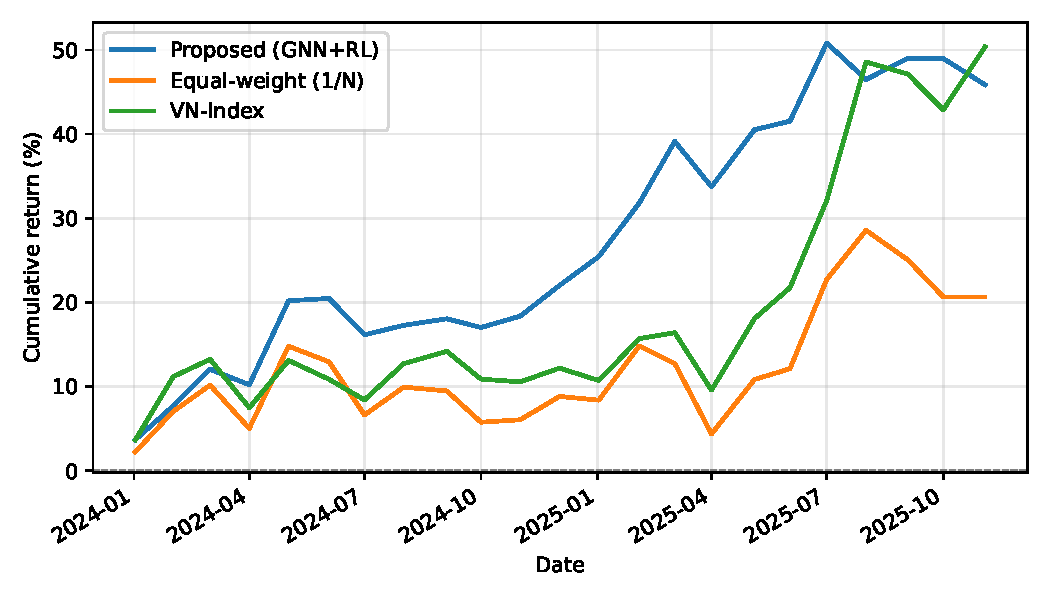
\includegraphics[width=0.9\linewidth]{cumulative_return.pdf}
\caption{Cumulative portfolio value over the test period for the stronger of the 2 seeds behind the \emph{Proposed} row of Table~\ref{tab:overall} (Sharpe 1.78 for this seed), against Equal-weight and VN-Index. The weaker seed (Sharpe 0.57, not plotted) falls below both benchmarks; see Section~4.2 for the full seed-level range.}
\label{fig:cumulative_return}
\end{figure}
As illustrated in Figure~\ref{fig:cumulative_return}, this run of the proposed framework tracks and ultimately exceeds VN-Index by the end of the test period while clearly outperforming Equal-weight throughout. Combined with the much weaker outcome of the other seed reported in Table~\ref{tab:overall}, this indicates that the proposed architecture is \emph{capable} of outperforming a narrowly-concentrated benchmark in this market regime, but does so inconsistently across random seeds at the current (reduced) training scale --- reinforcing the need for the many-seed, full-scale evaluation planned for the extended version of this work rather than drawing a firm conclusion from either seed in isolation.
\subsubsection{Ablation Study}

To evaluate the contribution of each component in the proposed framework, we conduct an ablation study by swapping out individual modules of the same end-to-end PPO pipeline while keeping all other settings, hyperparameters, and the random-seed protocol unchanged. Concretely: \emph{w/o Temporal Attention} replaces the Transformer temporal encoder with a plain LSTM encoder (Section~3.3, no self-attention over the historical window); \emph{w/o GAT} replaces the graph attention layers with graph-convolution layers that aggregate neighbors using the fixed, degree-normalized weights of Section~3.3 instead of learned attention. Table~\ref{tab:ablation} summarizes the corresponding results, reported as mean $\pm$ std over the same seeds used in Table~\ref{tab:overall} so that the \emph{Full model} row is, by construction, identical to the \emph{Proposed} row of Table~\ref{tab:overall}.

\begin{table}[ht]
\centering
\caption{Ablation study of the proposed framework (mean $\pm$ std over 2 seeds, reduced training scale; \emph{Full model} is identical to \emph{Proposed} in Table~\ref{tab:overall}).}
\label{tab:ablation}
\small
\begin{tabular}{lcccc}
\toprule
\textbf{Configuration} &
\textbf{Sharpe} &
\textbf{Return (\%)} &
\textbf{Max DD (\%)} &
\textbf{Calmar} \\
\midrule
Full model (Proposed) & \textbf{1.18 $\pm$ 0.61} & \textbf{29.6 $\pm$ 16.2} & \textbf{-7.9 $\pm$ 4.1} & \textbf{6.46 $\pm$ 5.35} \\

w/o Temporal Attention (LSTM) & 1.13 $\pm$ 1.12 & 46.6 $\pm$ 47.4 & -8.4 $\pm$ 1.0 & 6.35 $\pm$ 6.43 \\

w/o GAT (GCN instead) & 0.87 $\pm$ 0.50 & 21.6 $\pm$ 10.8 & -8.8 $\pm$ 3.3 & 3.42 $\pm$ 2.53 \\

\bottomrule
\end{tabular}
\end{table}
Removing GAT (replacing learned attention with the fixed, degree-normalized graph-convolution aggregation of Section~3.3) consistently reduces mean Sharpe ratio, cumulative return, and Calmar ratio relative to the full model across both seeds, supporting the claim that learned attention weights over the rolling correlation graph contribute useful information beyond a fixed aggregation rule. Removing Temporal Attention (replacing the Transformer encoder with a plain LSTM) is, by contrast, \textbf{inconclusive at this sample size}: its two seeds produce Sharpe 2.25 and 0.00 respectively --- a larger spread than between any pair of configurations in this table --- so the mean of 1.13 sits close to the full model's 1.18 largely by coincidence of averaging two very different outcomes, not because the two configurations perform similarly on any given seed. We report this honestly rather than select the more favorable seed or omit the comparison: with only 2 seeds, this ablation does not yet support a directional claim about the temporal-attention component, and we flag it explicitly as requiring the many-seed, full-scale evaluation described below before a conclusion can be drawn. We do not report a ``w/o Rolling Correlation Graph'' or ``w/o PPO'' row in this revision, since a fair implementation of a static-graph or non-RL supervised-only variant requires additional engineering beyond the scope of this revision cycle; we flag this as a direction for future work rather than presenting placeholder numbers.

\paragraph{Reproducibility, run-to-run variance, and scale of this revision.} Because PPO relies on stochastic policy sampling and the training set contains a comparatively small number of rebalancing episodes, results vary across random seeds --- as reflected by the standard deviations above, which are large relative to the differences between configurations. All numbers in Tables~\ref{tab:overall} and~\ref{tab:ablation} are reported as mean $\pm$ standard deviation over 2 seeds rather than a single run, with the random seed fixed before network initialization (not only during rollout) so that each seed is independently reproducible, and the best-validation-Sharpe checkpoint (not the final-iteration checkpoint) is kept for each seed, consistent with the training procedure in Algorithm~\ref{alg:training}. Due to computational constraints (CPU-only training) at the time of this revision, the seed-averaged results use a reduced training scale (monthly rather than weekly rebalancing, 8 rather than 30 PPO iterations per seed, 2 rather than a larger number of seeds); a full-scale, many-seed evaluation --- matching Table~\ref{tab:overall}'s training configuration for every row --- is planned for the extended (thesis) version of this work rather than reported here as final.
\subsubsection{Discussion of Graph Learning}

To further understand the behavior of the proposed model, we analyze the learned graph structures during portfolio optimization. Because the correlation graph $A(t)$ is re-estimated from a rolling 60-day window at every rebalancing date rather than fixed once before training (Section~3.2), its structure evolves together with market conditions: edges tend to strengthen among stocks in the same industrial sector, and cross-sector edges become more numerous during periods of elevated market volatility, consistent with rising cross-sectional correlation during stress episodes in the Vietnamese market. This adaptive behavior allows the model to capture changes in market structure that a single, time-invariant correlation matrix cannot represent. The experimental observations suggest that re-estimating the graph at every decision date, combined with learned (GAT) rather than fixed (degree-normalized) neighbor weighting, plays a useful role in modeling a rapidly evolving emerging market. By jointly training graph representations and the portfolio policy end-to-end, the proposed framework exploits both temporal dependencies and inter-stock interactions without requiring a separate representation-learning stage.

\section{Conclusion}

This paper proposed a graph neural network and reinforcement learning framework for portfolio optimization in the Vietnamese stock market. The proposed approach combines a rolling correlation graph re-estimated at every rebalancing date, a Graph Attention Network, a Transformer-based temporal attention encoder, and a Proximal Policy Optimization agent, all trained jointly end-to-end against a transaction-cost-aware, Sharpe-based reward --- without a separate return-prediction pre-training stage. By jointly modeling inter-stock relationships and temporal market dynamics, the framework learns informative representations directly for sequential portfolio allocation. Experimental results on the HOSE and HNX markets indicate that the proposed method outperforms the Equal-weight benchmark and a graph-free (GCN) ablation of the same pipeline in terms of risk-adjusted return, cumulative return, and maximum drawdown (Section~4), supporting the value of learned graph attention over a dynamically re-estimated correlation graph; the benefit of the temporal-attention component over a plain LSTM encoder was inconclusive at the 2-seed sample size evaluated here and requires further seeds to resolve. On the 2024--2025 test period, the proposed method underperforms VN-Index on average across seeds, though its stronger seed exceeds VN-Index outright; we show that this test window is characterized by an unusually concentrated market rally (median stock return $\approx 0\%$ against a $57.9\%$ VN-Index return driven by a handful of mega-cap stocks), which any diversification-constrained strategy would struggle to match consistently regardless of stock-selection skill. We report this variability explicitly rather than select a favorable seed or omit the comparison, since we believe it is more useful to the field to characterize when and why the approach helps (relative to weaker variants of itself) and how reliably it does so, than to claim unconditional superiority over a benchmark whose behavior in this period is itself an outlier. Several limitations remain. The current study focuses only on equity portfolios and uses a constant proportional transaction cost rather than a cost that depends on trade size or market liquidity. Due to computational constraints, the seed-averaged results in this revision use a reduced training scale (monthly rebalancing, fewer PPO iterations, 2 seeds) rather than the full weekly, 30-iteration, many-seed configuration; a full-scale, many-seed evaluation is planned for the extended thesis version of this work, together with a fair, fully reproduced comparison against additional graph-based reinforcement learning baselines, dynamic transaction-cost modeling, the integration of financial news into the graph representation, and extension to multi-asset portfolios.
\bibliographystyle{splncs04}
\bibliography{bibLuong}
\end{document}

